% !Mode:: "TeX:UTF-8"


\chapter{引言}
\label{ch:intro}

根据天津大学模板修改的符合中山大学毕业论文(至少是硕士论文)要求的Latex模板。

\section{使用方法}
\label{sec:usage}

本模板只包括内容方面的设计预定义,编译自行解决。作者使用的是Windows环境下MikTex+TeXstudio的组合。

\section{使用建议}
\label{sec:tips}

\subsection{普适问题}
\label{subsec:common}

普遍适用的论文排版问题:

\begin{itemize}
\item 图片标题在下,表格在上;一定要有标题,不能只是图1-1;与文字内容的间隔自行把握。
\item 参考文献建议使用.bib文件;也有使用Google Scholar的引用的,但有指出当中的“//”不符合规范。
\item 部分评审反馈,目录不包含摘要及目录本身,请根据情况自行斟酌。
\item 打印时需要右边翻页的问题(每章开始在右边页),可以在生成pdf后通过插入空白页解决(这样插入不会改变页码);或者尝试设置openright (未测试,有待探讨)。
\end{itemize}

\subsection{细节问题}
\label{subsec:specs}

一些细节的问题建议:
\begin{itemize}
\item 每个章节都有label,key使用ch:intro形式,以下使用sec:background等。图片key可以参考fig:scenes,表格参考tab:exp。
\item 图片、表格尽量在页的顶部,即float优先选择t。
\item 另外,为了打印时彩打方便,可以把需要彩打的图片尽量排版在一页,不过比较难调。
\item 虽然每个body的tex文件中包含了!Mode:: ``TeX:UTF-8"在文件开头,但仍有必要在IDE中将新建的tex文件设为UTF-8 编码,否则可能无法正常显示中文。
\end{itemize}

\subsection{其他说明}
\label{sec:setting}

参考文献\cite{wu2013online}目前采用上标表示。使用cite命令。

目前页眉设置:每章第一页页眉只有中间的“中山大学硕士毕业论文”,后续页左边显示“中山大学硕士毕业论文”,右边显示“第n章”。

目前页脚设置:仅包含页码,居中,无横线。

参考文献和附录计算页数,包含在目录,页眉设置同每章第一页。正文前的部分无页眉。

\section{例子}
\label{sec:examples}

图例子。label要在caption后。多图或子图方法上网查吧。

\begin{figure}[!t]
	\centering
	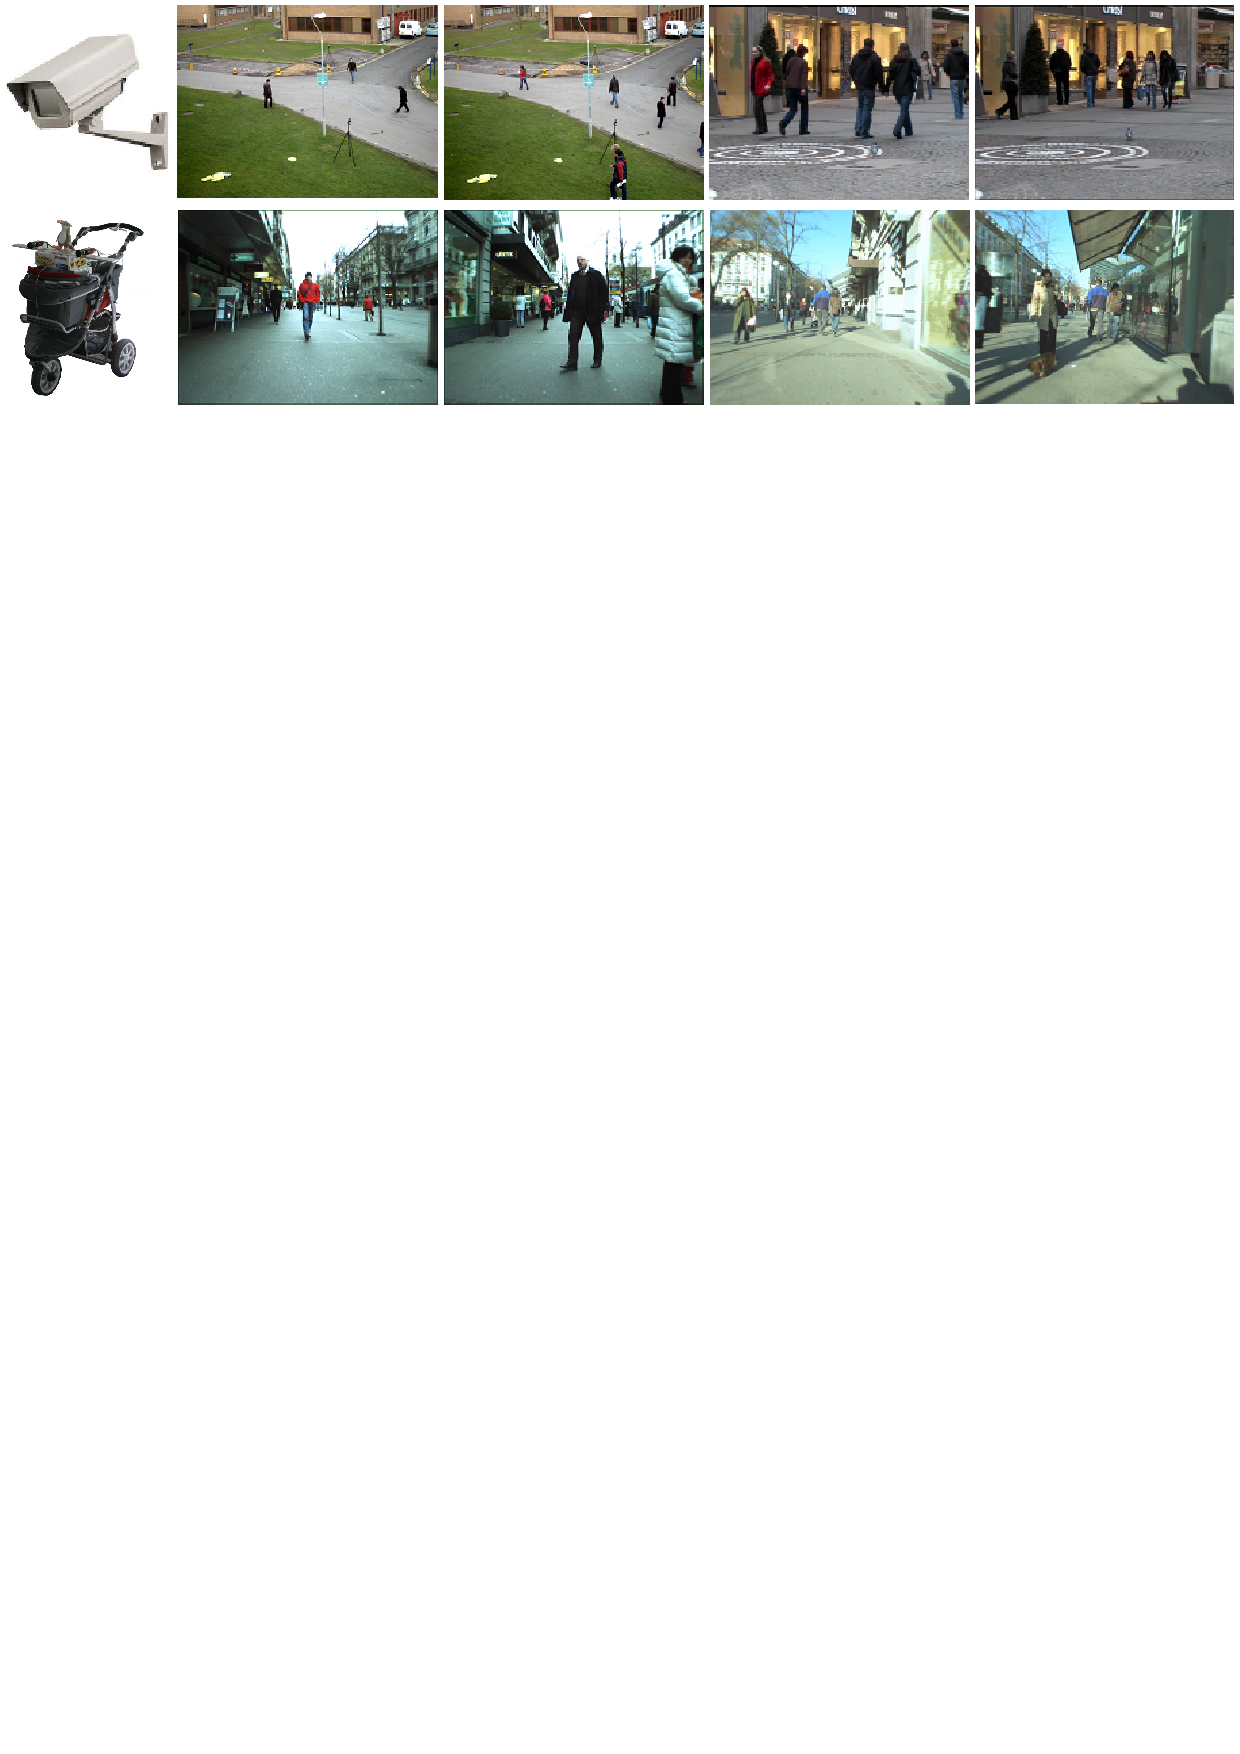
\includegraphics[width=0.95\textwidth]{scenes}
	\caption{图例}
	\label{fig:scenes}
\end{figure}

表例子。推荐使用这种三行表。缺省值使用三个“-”产生长横线“---”。

\begin{table}[!t]
\caption{示例表}
\label{tab:eg}
\vspace{0.5em}
\centering
\wuhao
	\begin{tabular}{ccccc}
	\toprule[1.5pt]
	表头 & 栏1 & 栏2 & 栏3 & 栏4 \\
	\midrule[1pt]
	内容1 & b & --- & $768 \times 576$ & 19 \\
	内容1 & a & 240/7 & $768 \times 576$ & --- \\
	\bottomrule[1.5pt]
	\end{tabular}
\end{table}

公式例子,与普通Latex数学公式无异。

\begin{equation}
1+1=2
\end{equation}

\subsection{研究背景和意义}

每个人的社会关系从构成了我们日常生活中社会结构的基础。自然的,我们利用一个人所在场景的社会关系来理解和解释当前的场景。社会学研究表明,这种对人的社会理解允许对其特征和可能的行为进行推断。当前,我们的社交生活很大部分是在社交媒体上,例如Facebook、Twitter、微信和微博等包含多模态信息的App,人们会通过文字、视频和音频等媒介含蓄的留下一些痕迹,但是我们能明确的扑捉到他们的社会关系通过分析多模态的信息。随着科技的发展和未来的到来,智能和潜在的自主系统会成为我们的帮手和同事,我们希望它们不仅可以熟练的完成任务,还希望他们能够融入和在我们人类生活的不同情况下采取适当的行动。此外,通过更好地了解这些隐藏信息,我们希望告知用户潜在的隐私风险。理解社会关系也有助于避免潜在的隐私风险,通过自动分析可能在文本等许多媒体中揭示社会关系的信息并告知用户这一点。在这个模式中,任务要求社会关系的概念和模式需要在生活和的所有方面共同努力,以便从一种感觉到的输入。虽然已经开始努力解决这一具有挑战性的问题,但社会生活的巨大多样性和复杂性阻碍了进展。最常见的,识别社会关系的计算模型仅仅限定于少数特定的类别。

在图像理解任务上,视觉概念识别获得了越来越多的研究者的关注,包括视觉属性和视觉关系\cite{lu2016visual}。
视觉关系和视觉属性检测的主要目的是构建场景图谱,场景图谱(scene graph)\cite{johnson2015image}是对图片进行描述的一种半结构化的形式,场景图谱是由视觉三元组构成,并且包括关系三元组和属性三元组。场景图谱已经成为计算机视觉和人工智能领域的重要基础资源,因此如何自动的构建场景图谱成为了重要关注点,以利用自然语言信息的\cite{lu2016visual}为代表的工作,代表场景图谱自动生成领域取得了极大的进展。同样,社会属性和社会关系\cite{wang2010seeing} 对于场景理解同样重要。因此在当前工作,主要聚焦在解决社会关系检测问题上,并且可以从场景图谱的生成借鉴有用的思想。
给定一张图片,社会关系理解的目的是推断在当前图片这个场景下人之间的社会关系是社会关系检测的准确描述。除了前面提的用处,理解图像场景中这样的关系能帮助现有的算法产生更好的场景描述。例如在图\ref{fig:intro-example}中的第一个样例,用正常的文字来描述的话,`` 一个妇人和女孩正在吃饭''。但是对于社会关系的这个问题下,可以认为是``一个母亲和女儿正在吃饭''。
\begin{figure}[htpb]
	\centering
	%	\includegraphics[width=0.48 \textwidth, trim=10 10 10 80,clip]{./pic/example_new.pdf}
	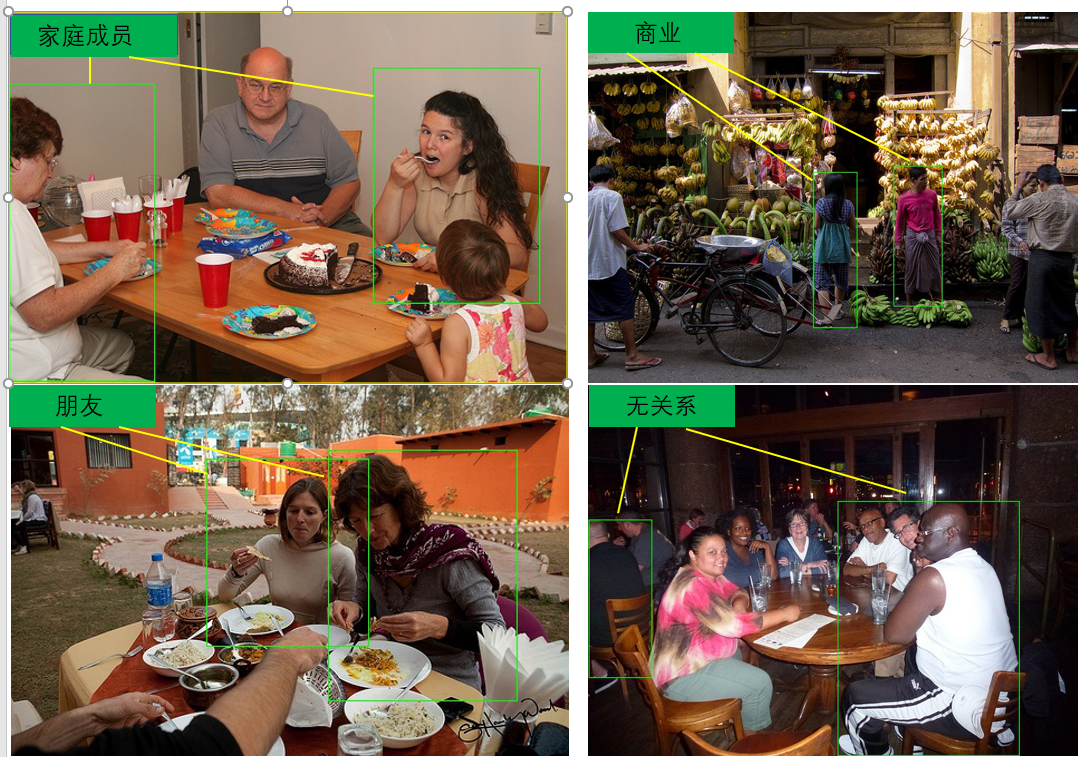
\includegraphics[width=0.95 \textwidth,clip]{example-1.png}
	%\hspace{0.02\textwidth}
	%\vspace*{-0.08cm}
    \caption{PISC数据集中的一些图片例子}
	\vspace*{-3.5mm}
	\label{fig:intro-example}
\end{figure}
\looseness=-1

既然社会关系理解对于理提升上述任务的关键资源,那么自然而然的,如何准确的理解社会关系成为需要研究者需要攻克的课题。一方面,一张图片的社会关系可以通过众包的方式,人工标注得到,比如现有的数据集PISC\cite{li2017dual-glance}和PISC-relation\cite{sun2017a}。当然,自动端到端的方法包括基于人脸特征、年龄、人的头部特征等特征信息的\cite{sun2017a,zhang2015learning}。还有利用周边环境的信息的模型\cite{li2017dual-glance,wang2018deep},这些模型通常需要一个物体检测器或者检测器中RPN(region proposal network),这都是需要引入额外的标注框或者预训练模型。也有通过对周边物体和社会关系共现的统计,例如``computer''和``professional''共同出现的概率较大,如果识别出存在``computer'',那么当前的关系很大概率是``professional'',通过神经网络引入这些先验知识来提升预测的准确率。这些自动识别社会关系的模型虽然不断在进步,但是从实验结果来看,他们与人工标注的准确率还是存在很大鸿沟,离实际的应用还存在很大的距离。

然后,现有的学习模型大都倾向于利用外部的知识来辅助理解图片的社会关系场景,但是得到这些外部知识需要额外的人工标注,这是一件耗时耗力的工作,或者一些统计得到的先验知识同样包含一些噪音,这也直接引出了到底是否应该引入外部知识,例如是否利用周边物体的信息,以及如何在缺乏这些信息的情况下取得好的实验效果。受到场景图谱生成的启发,场景图谱的概念最初是在2015年由Johnson 等人\cite{johnson2015image}提出的,是用于描述图片的一种新的半结构化的方式,基本组成单位是视觉三元组,形式为(头实体,关系,尾实体)。受到该领域下xu(2017)\cite{xu2017scene}的工作首先将整张图片输入,考虑到图片中不同视觉三元组之间的相互影响。例如,当知道``马在草地上''倾向于提高检测到``人骑着马''这条视觉三元组。对于社会关系检测的场景,如果图片中包含三个人对,其中两个人对的社会关系是``朋友'',那么第三条关系的的社会关系会倾向也是``朋友''或者其他的亲密关系,而不是``无关系''。直观上来说,这个是成立的,因此我们可以利用这当前场景下的其他的关系的来推理出当前的关系。

本论文主要研究如何将前文提到的关系场景的上下文信息引入社会关系理解的框架中。本论文完全区别于Li(2017)\cite{li2017dual-glance}和Wang(2018)\cite{wang2018deep}的工作,没有引入额外的检测标注
,但是采用和Li等特征提取方法相同的策略。论文的切入点如图例\ref{fig:intro-example-2},图上六个人对的关系有五对是``朋友''关系,其中只有一对``奶奶-孙女''的关系,因此当前的图片应该是一个朋友聚会的场景拍下的。如果我们想推理出其中一个人对的关系并且已经知道其他部分人对的关系,那么直观的,我们会通过对已经知道的关系进行一个场景的判断,从而推理当前人对的关系到底是什么。在当前例子中,如果已经知道了2对或者3对都是``朋友''关系,那么当前的人对大概率也是``朋友''关系。因此,类似于前文提到的场景图谱的生成,以及现有的社会关系理解的研究现状,将当前的工作成为社会关系图谱生成
(social graph generation)。
\begin{figure}[htpb]
	\centering
	%	\includegraphics[width=0.48 \textwidth, trim=10 10 10 80,clip]{./pic/example_new.pdf}
	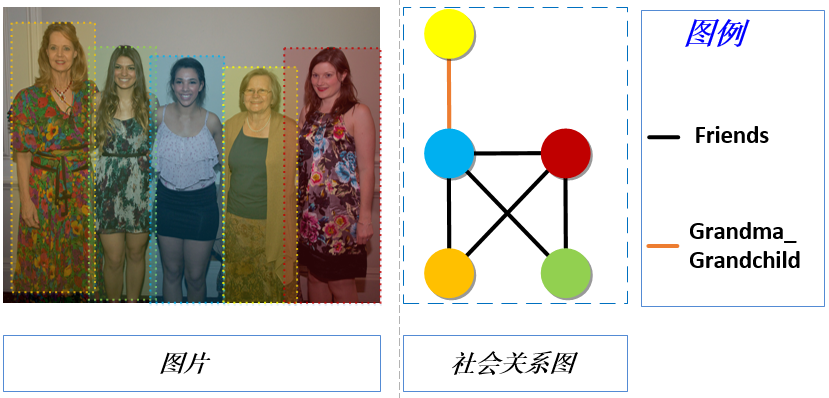
\includegraphics[width=0.95 \textwidth,clip]{example-2.png}
	%\hspace{0.02\textwidth}
	%\vspace*{-0.08cm}
    \caption{本论文动机的示例图,该图片来自PIPA-relation数据集,其中图片中对应阴影颜色的人对应社会关系图的部分,图上节点间的边表示他们之间的社会关系}
	\vspace*{-3.5mm}
	\label{fig:intro-example-2}
\end{figure}
\looseness=-1

在上述的介绍中,我们分别提到了两方面的相关内容,一方面社会关系理解的意义和作用,另外提到了与社会关系同属视觉理解领域的场景图谱的生成,收到这些工作的影响,可以列出他们的共性和特性如下:
\begin{enumerate}
    \item 场景图谱的基本组成是视觉三元组,社会关系图中是人对和人对间的社会关系,但是场景图谱中并没有人的的类别的概念,社会关系图中节点间的社会关系与人的类别无关。
    \item 场景图谱中的关系类别较多,有80-100个类别,但是在社会关系中,现有数据集不同粒度的关系类别分别为3、6、16,数量上远远不一样。并且在场景图谱中,关系的类型主要以空间关系为主,少量含有语义的关系,但是在社会关系图中,除了``无关系''和空间存在较大关联,其他的均为语义的关系。
    \item 与现有研究工作的区别是,之前的方法均将同一张图片上的不同人之间的关系割裂来看,但是他们间的关系互相影响,现有的研究工作忽略了这一点。
\end{enumerate}

要想解决社会关系理解问题,一种可行的方法是借助场景中除了人以外其他的信息,由于现有的数据集并没有标注其中的物体信息,所以需要借助额外的检测模型,但是由于模型的准确率的原因,会引入相当一部分的噪音,我们不能简单的加入这些信息,或者说我们是否需要加入这部分信息。其次是借助场景图谱生成的思想,认为一张图片中所有人对的社会关系不是割裂开的,是一同生成的,并且它们之间是相互影响的,但是由于场景图谱和社会关系图的区别,我们需要设计一个在社会关系理解人物下人对关系之间的交互机制。

\section{研究现状}

\subsection{视觉关系理解的应用}
在计算机视觉领域,社会关系信息被探索来提升几个常见的任务,例如人的轨迹预测\cite{kim2015brvo,robicquet2016learning}、 多目标追踪\cite{chen2012discovering,qin2012improving}和群体活动识别
\cite{direkoglu2012team,lan2012social,lan2012discriminative}。例如,在Deng等人(\cite{deng2016structure})群体活动识别的任务中,群体活动识别需要推理出图上人之间的结构信息,当前的方法是判断每个个体的动作,并且判断图上人之间的关系。但是由于图片特征的复杂和不确定性,这两个任务都是很有挑战的,推断出图上的结构信息能帮助排除一些未参与群体活动的人,得到更好的预测结果。因此预测这些人之间的社会关系能有助于群体活动识别。如图例\ref{fig:deng-example}所示,利用深度学习模型得到的人的表征和场景的表征后,如果知道了图例中第三个人和另外两个人之间不存在关系的情况下,排除第三个人对任务判断的影响。能更为容易的得出当前的群体活动场景是``waiting''。如Alahi 等人(2016)\cite{alahi2016social}隐含的引入了社会性的约束来预测符合社会常识规则的人类轨迹。
\begin{figure}[htpb]
	\centering
	%	\includegraphics[width=0.48 \textwidth, trim=10 10 10 80,clip]{./pic/example_new.pdf}
	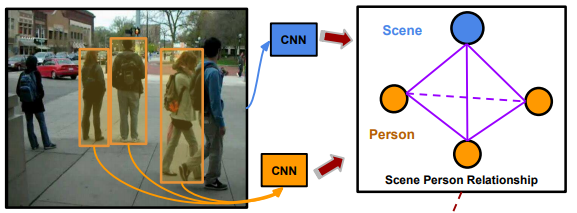
\includegraphics[width=0.95 \textwidth,clip]{deng-example.png}
	%\hspace{0.02\textwidth}
	%\vspace*{-0.08cm}
    \caption{来自Deng等人\cite{deng2016structure}的示例图}
	\vspace*{-3.5mm}
	\label{fig:deng-example}
\end{figure}
\looseness=-1

前面的工作大多数都是利用向量化的社会关系来帮助推理,与社会关系理解同属同一个视觉关系理解任务类别,即场景图谱的生成,又或者称为视觉关系检测。该任务的最早是Johnson等人于2015年提出的
\cite{johnson2015image},是一种用于描述图片场景的新的方式,与本文工作不同的是,场景图谱中的主要组成部分不仅包括人,还包括很多日常物体,如图\ref{sg-example}所示。两个工作最核心的挑战在于推理出物体之间的关系。由于场景图谱常用于图片检索\cite{johnson2015image},Marino(2017)\cite{marino2017the}利用得到场景图谱结合图神经网络提高图片的分类效果。在以上关于视觉信息理解的两个方向上,都有大量的工作提出,分别用于解决不同场景的问题,因此如何更好的实现视觉理解这个难题自然而然的成为许多研究者想要攻克的难题。对于场景图谱来说,本文的工作主要受到了一下几个工作的启发。Xu等人(2017)对于场景图谱进行建模,分别包含物体节点和关系节点,然后采用Message Passing的方式进行迭代。通过相邻的节点或边对目标节点或边进行约束,从而对这些特征进行微调,达到提升的效果。Yang等人(2018)利用图卷积网络进行不同节点之间的Message passing来达到约束的效果。\cite{liang2018visual}利用自然语言指导提出的VRD模型,本文初始步骤的特征提取工作中包含空间信息的提取便收到该工作的启发。
\begin{figure}[htpb]
	\centering
	%	\includegraphics[width=0.48 \textwidth, trim=10 10 10 80,clip]{./pic/example_new.pdf}
	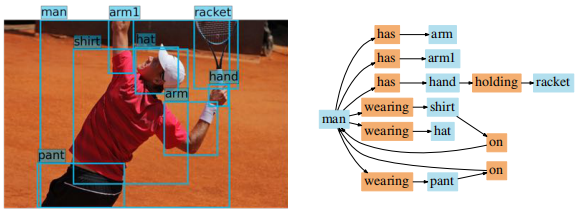
\includegraphics[width=0.95 \textwidth,clip]{sg.png}
	%\hspace{0.02\textwidth}
	%\vspace*{-0.08cm}
    \caption{场景图谱\cite{xu2017scene}的示例图}
	\vspace*{-3.5mm}
	\label{fig:sg-example}
\end{figure}
\looseness=-1

\subsection{社会关系理解的方法}
而对于社会关系理解,作为最早的工作,wang等人(2010)开始引入家庭关系当前背景来识别人之间亲属关系。在后来的工作中\cite{dibeklioglu2013like,xia2012understanding,chen2012discovering},为了捕获这些社会关系展现出来的一些规律,探索了面部表情和属性等用于亲属关系识别和验证。并且为了促进社会关系理解领域的研究和发展,Li\cite{li2017dual-glance}和Sun\cite{sun2017a}构建了大规模的数据集,并且利用深度学习的模型直接从图片中学习来识别关系。对于Sun构建的数据集PIPA-Relation,该数据集的关系包括5个领域,然后基于这5个领域又划分为16条关系。同样,Li基于关系模型理论,定义了一系列的关系列别,包含两类关系的划分,粗粒度的3类关系和细粒度的6类关系。
\subsection{本文工作}

本文首先通过介绍现有的社会关系理解的最新研究工作,分析它们的模型设计的出发点,模型的结构,分析这些工作的忽略的信息,即没考虑到整张图片不同的人对的关系之间的互相影响。因此,本文提出了一个考虑到同一张图片不同关系之间存在交互的模型:包含人对消息传递机制的模型,人对关系网络(Person-pair Relation Network),简称PPRN,最后把该模型应用到社会关系理解的任务中,在两个公开数据集上做了对比实验。
本文提出的PPRN模型包括以下三个模块:
\begin{enumerate}
    \item 特征抽取模块,
    \item 消息传播模块
    \item 消息池化模块
\end{enumerate}


